\subsection{\ac{COBE}}
Die \ac{COBE} Mission, hatte den Zweck, exakte 
Messungen der kosmischen Infrarot-(hier nicht näher behandelt) und 
Mikrowellenhintergrundstrahlung durchzuführen.
Der Satellit wurde am 18. November 1989 ins All geschossen und verfügte über 
drei Messinstrumente \cite{cmb:COBE}:
\begin{itemize}
	\item \ac{DIRBE}: Um nach der 
	kosmischen Infrarotstrahlung zu suchen.
	Dank der Messung dieser Strahlung konnten unter anderem Modelle der 
	Entstehung von Sternen erstellt werden.
\index{DIRBE}%
\index{diffuse infrared background experiment}%
	\item \ac{DMR}: Um die Anisotropie der 
	kosmischen Hintergrundstrahlung nachzuweisen.
\index{DMR}%
\index{differential microwave radiometer}%
	\item \ac{FIRAS}: Um die Temperatur 
	der kosmischen Hintergrundstrahlung nachzuweisen. 
\index{FIRAS}%
\index{far-infrared absolute spectrometer}
\end{itemize}

Das Resultat dieser Messungen ist in Abbildung~\ref{fig:COBE} zu sehen.
\begin{figure}
	\centering
	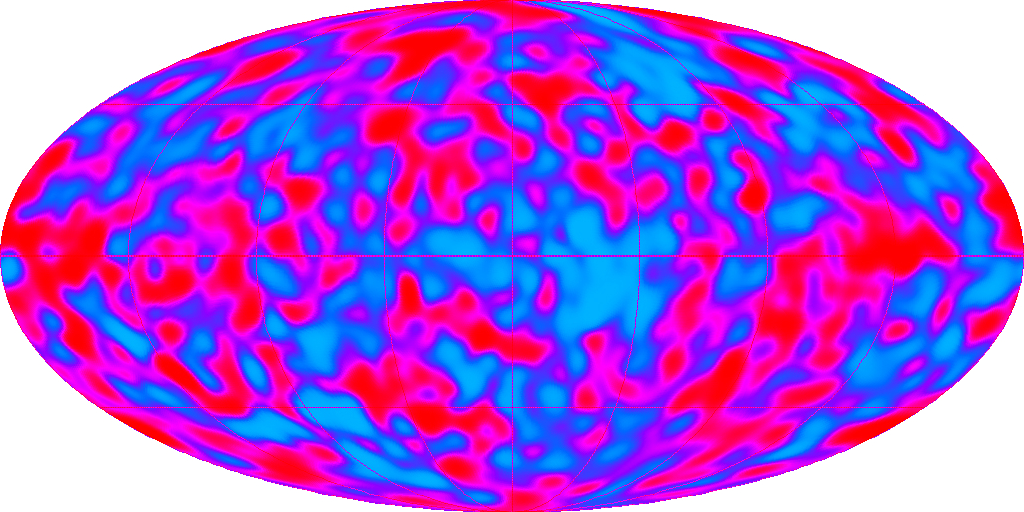
\includegraphics[width=\linewidth]{cmb/images/CMB_COBE.png}
	\caption{Das erste Bild der kosmischen Hintergrundstrahlung.}
	\label{fig:COBE}
\end{figure}
Die \ac{COBE} Mission war ein voller Erfolg.
Die letzten Zweifel an der Urknall-Theorie konnten zerstreut werden.
\ac{DMR} konnte Temperaturschwankungen zwischen verschiedenen Stellen am Himmel 
von $10^{-5} \text{K}$ nachweisen, womit die Anisotropie der Strahlung bewiesen 
war.
\ac{FIRAS} mass den spektralen Verlauf der Strahlung und kam zum Ergebnis, dass 
ihre Temperatur von $2.725 \text{K}$ extrem genau der eines Schwarzkörpers 
entspricht (siehe Abbildung~\ref{fig:CMB_spectrum}).
Damit war bewiesen, dass es sich bei der gemessen Strahlung tatsächlich um die 
kosmische Hintergrundstrahlung handelt, da man weiss, dass eine zur 
Rekombination entstandene Schwarzkörperstrahlung sich von $3700 \text{K}$ auf 
eben diese $2.725 \text{K}$ abgekühlt haben muss.

John C. Mather (\ac{NASA}) und George F. Smoot (University of California), 
\index{Mather, John C.}%
\index{Smoot, George F.}%
erhielten
für ihre Arbeit an der \ac{COBE} Mission 2006 den Nobelpreis für Physik.
\begin{figure}
	\centering
	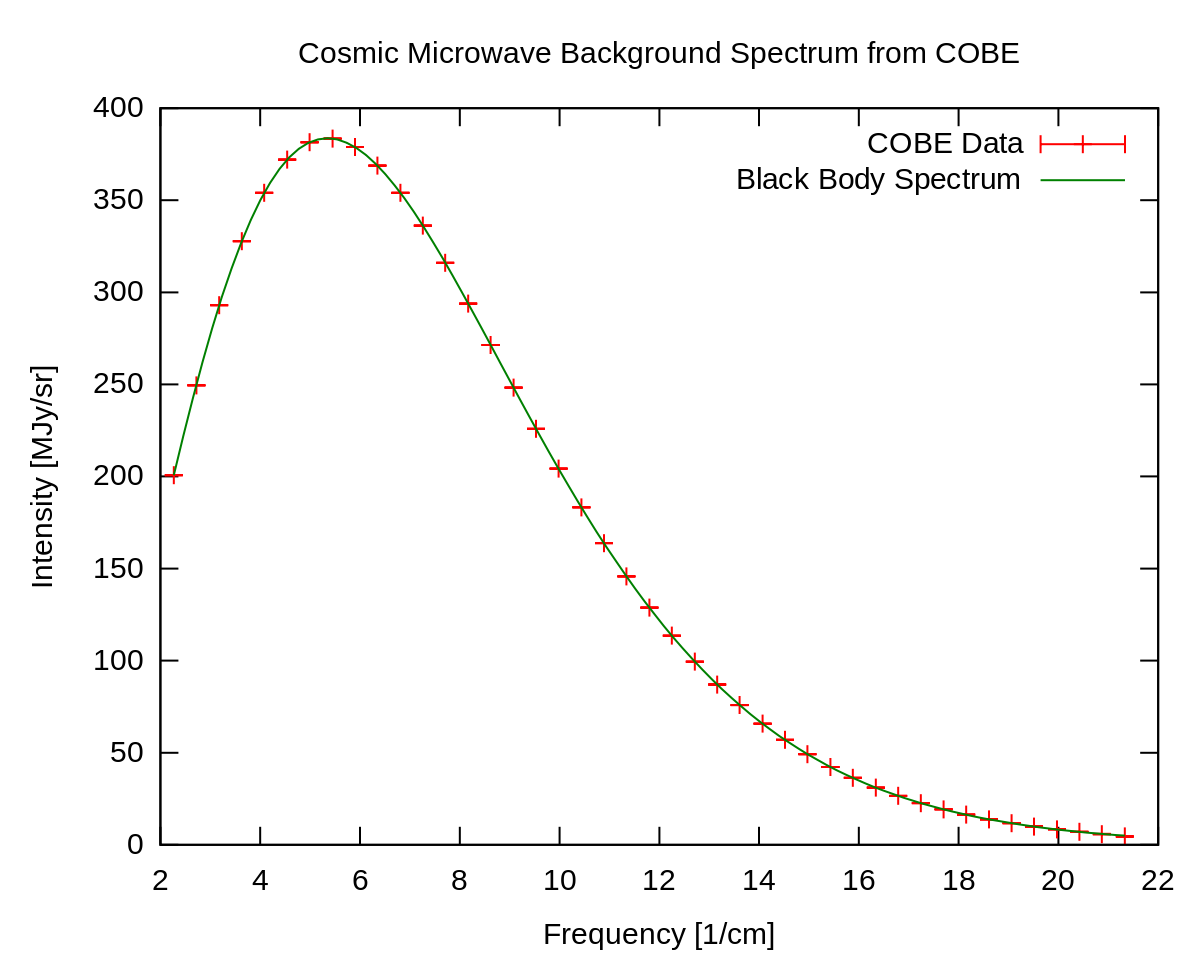
\includegraphics[width=0.7\linewidth]{cmb/images/CMB_spectrum.png}
	\caption{Das von \ac{COBE} gemessene Spektrum stimmt perfekt mit dem 
	erwarteten Schwarzkörper-Spektrum überein.}
	\label{fig:CMB_spectrum}
\end{figure}

\subsection{\ac{WMAP} und Planck}
\index{WMAP}%
\index{Wilkinson Microwave Anisotropy Probe}%
\index{European Space Agency}%
\index{Planck-Mission}%
\ac{WMAP} (\ac{NASA}) und Planck (\ac{ESA}) folgten auf 
\ac{COBE}.
Ihr Ziel war es unter anderem, präzisere Bilder der kosmischen 
Mikrowellenhintergrundstrahlung zu erhalten.

\subsubsection{\ac{WMAP}}
\ac{WMAP} wurde im Juni 2001 ins All geschossen, mit dem Ziel verschiedenste 
kosmologische Messungen durchzuführen.
Die Resultate dieser Messungen sind sehr vielfältig, deswegen werden die 
interessantesten hier kurz aufgeführt:
\begin{itemize}
	\item Messung der kosmischen Hintergrundstrahlung: Durch die \ac{WMAP} 
	Messungen konnte ein sehr exaktes Bild der Strahlung erzeugt werden (siehe 
	Abbildung \ref{fig:CMB_WMAP}).
	\begin{figure}
		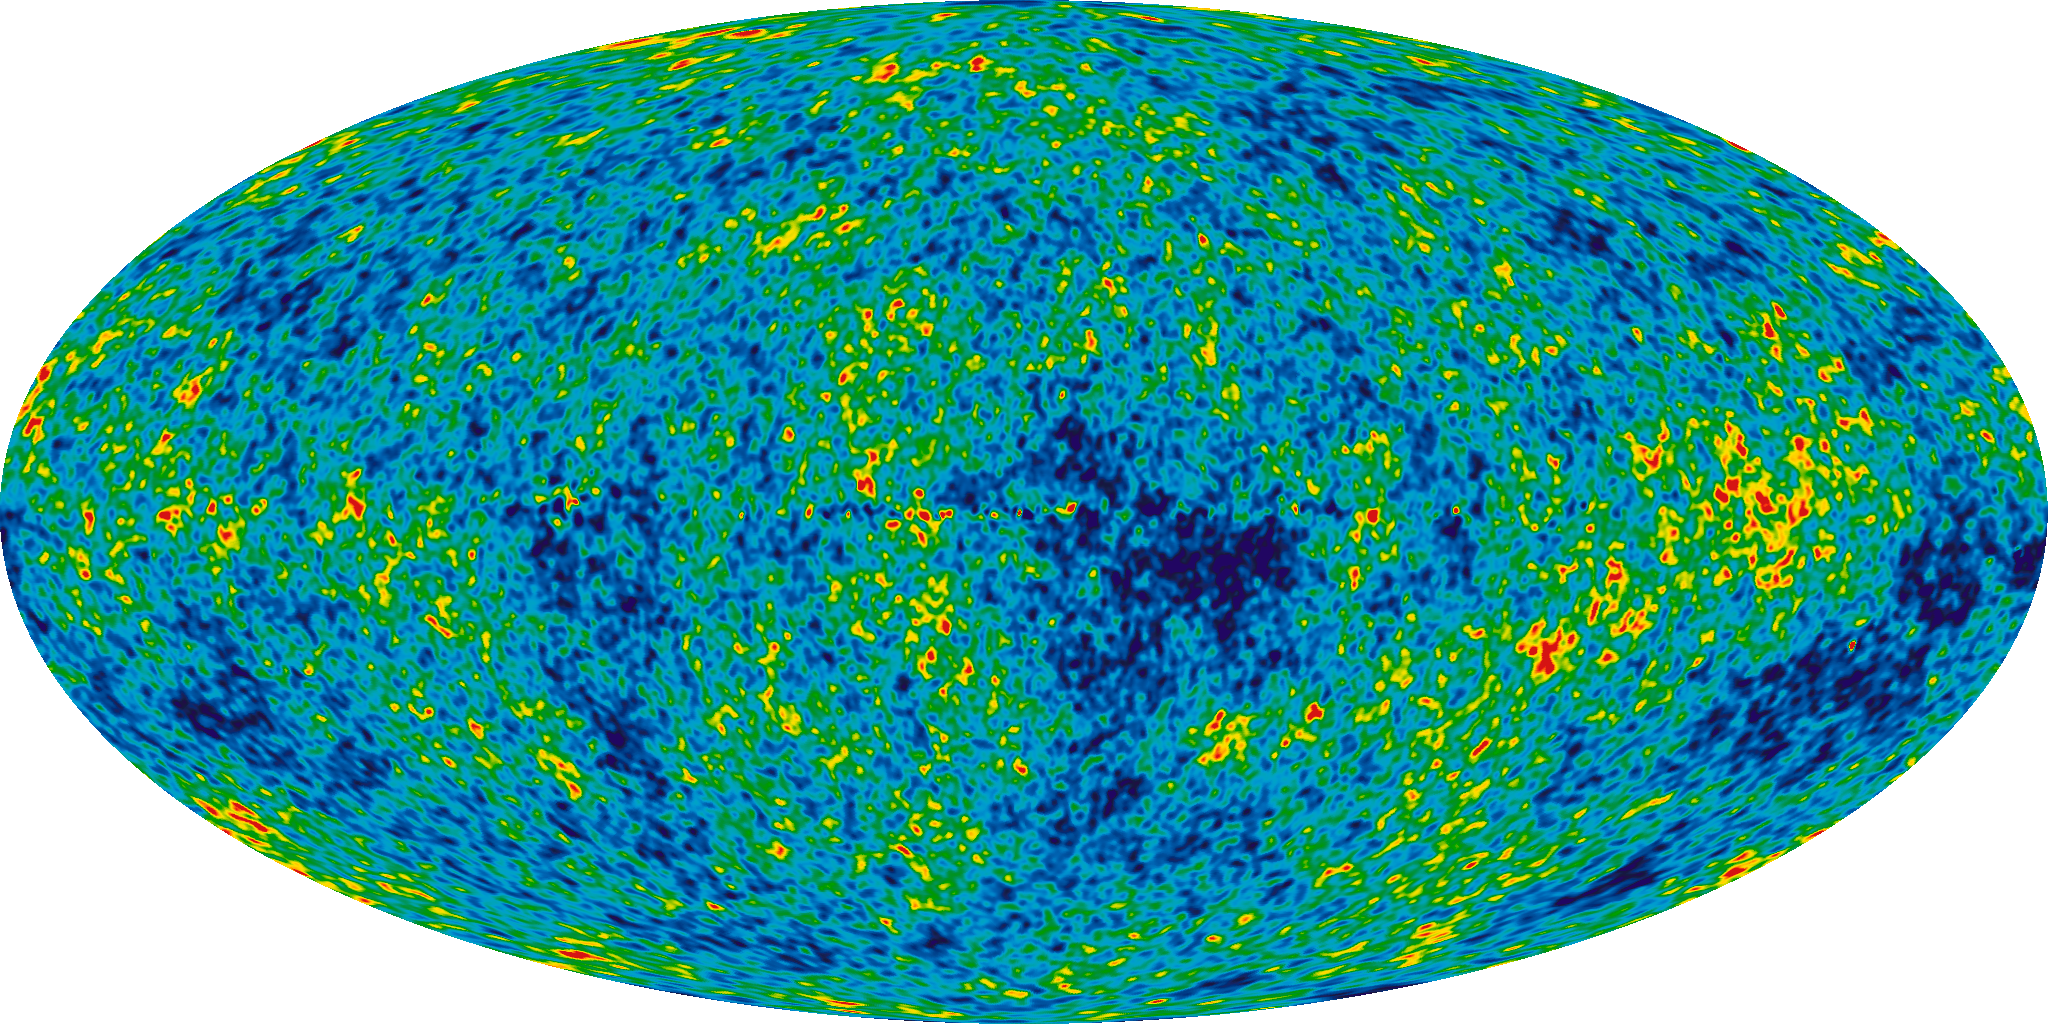
\includegraphics[width=\linewidth]{cmb/images/CMB_WMAP.png}
		\caption{Kosmischer Mikrowellenhintergrund gemessen von \ac{WMAP}.}
		\label{fig:CMB_WMAP}
	\end{figure}
	\item Alter des Universums: Das Alter des Universums konnte auf ein halbes 
	Prozent genau auf 13.77 Milliarden Jahre bestimmt werden.
	\item Dunkle Materie und dunkle Energie: Es konnte bestimmt werden, dass 
	das Universum zu $24.0 \%$ aus dunkler Materie und zu $71.4\%$ aus 
	dunkler Energie besteht.
\index{dunkle Materie}%
\index{dunkle Energie}%
\index{Energie, dunkle}%
\index{Materie, dunkle}%
\end{itemize}
Dies ist nur ein kleiner Ausschnitt aus den vielfältigen Resultaten der 
\ac{WMAP} Mission \cite{cmb:WMAP}.

\subsubsection{Planck}
Planck wurde 2009 abgeschossen, um die kosmische 
Mikrowellenhintergrundstrahlung noch genauer als bisher studieren zu können.
Das Ziel war es, das derzeitige Standardmodell des Universums so zu bestätigen, 
dass es über jeden Zweifel erhaben ist.
Aus den Daten konnte ein noch besser aufgelöstes Bild (siehe Abbildung 
\ref{fig:CMB_Planck}) generiert werden:
\begin{figure}
	\centering
	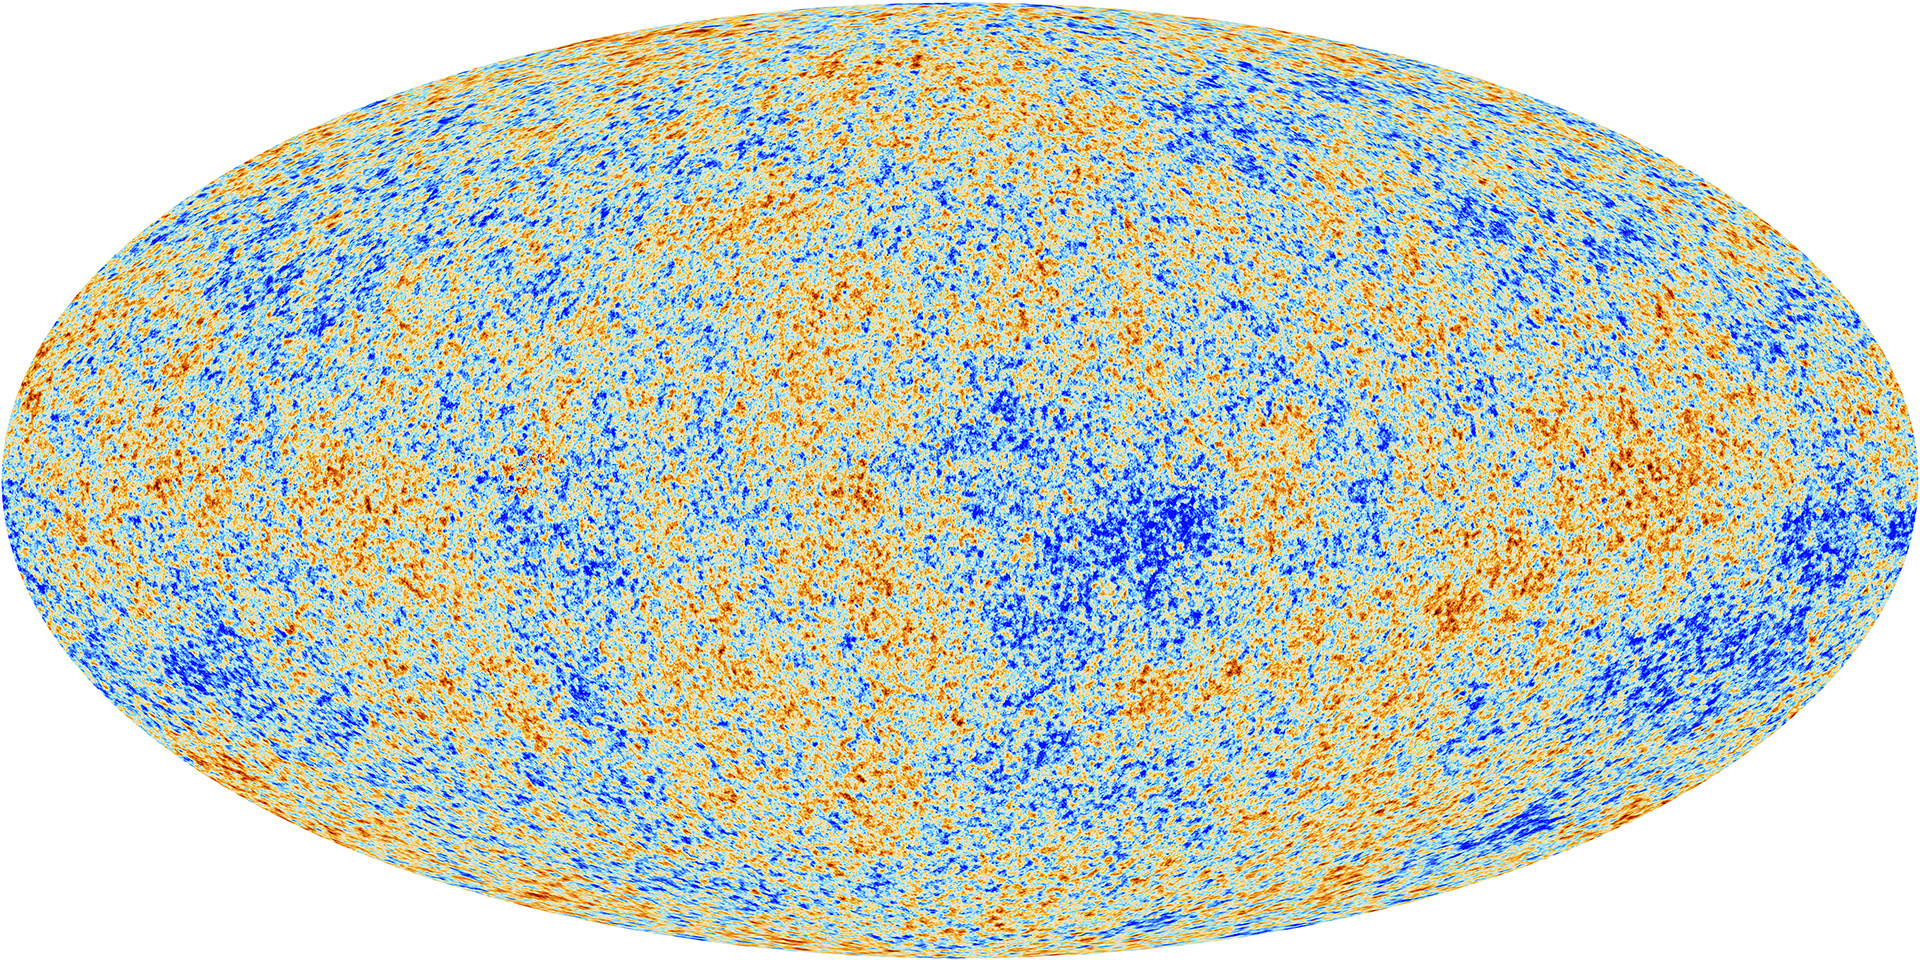
\includegraphics[width=\linewidth]{cmb/images/CMB_Planck.jpg}
	\caption{Kosmischer Mikrowellenhintergrund gemessen von Planck. (\copyright 
	ESA, Planck Collaboration)}
	\label{fig:CMB_Planck}
\end{figure}
Das Ziel von Planck wurde erreicht und das zurzeit anerkannte Modell konnte 
bestätigt werden.

\subsection{Vergleich}
Stellt man die Bilder im direkten Vergleich dar 
(Abbildung~\ref{fig:COBE_WMAP_PLANCK}), sieht man, wie stark die Auflösung 
verbessert wurde.
\begin{figure}
	\centering
	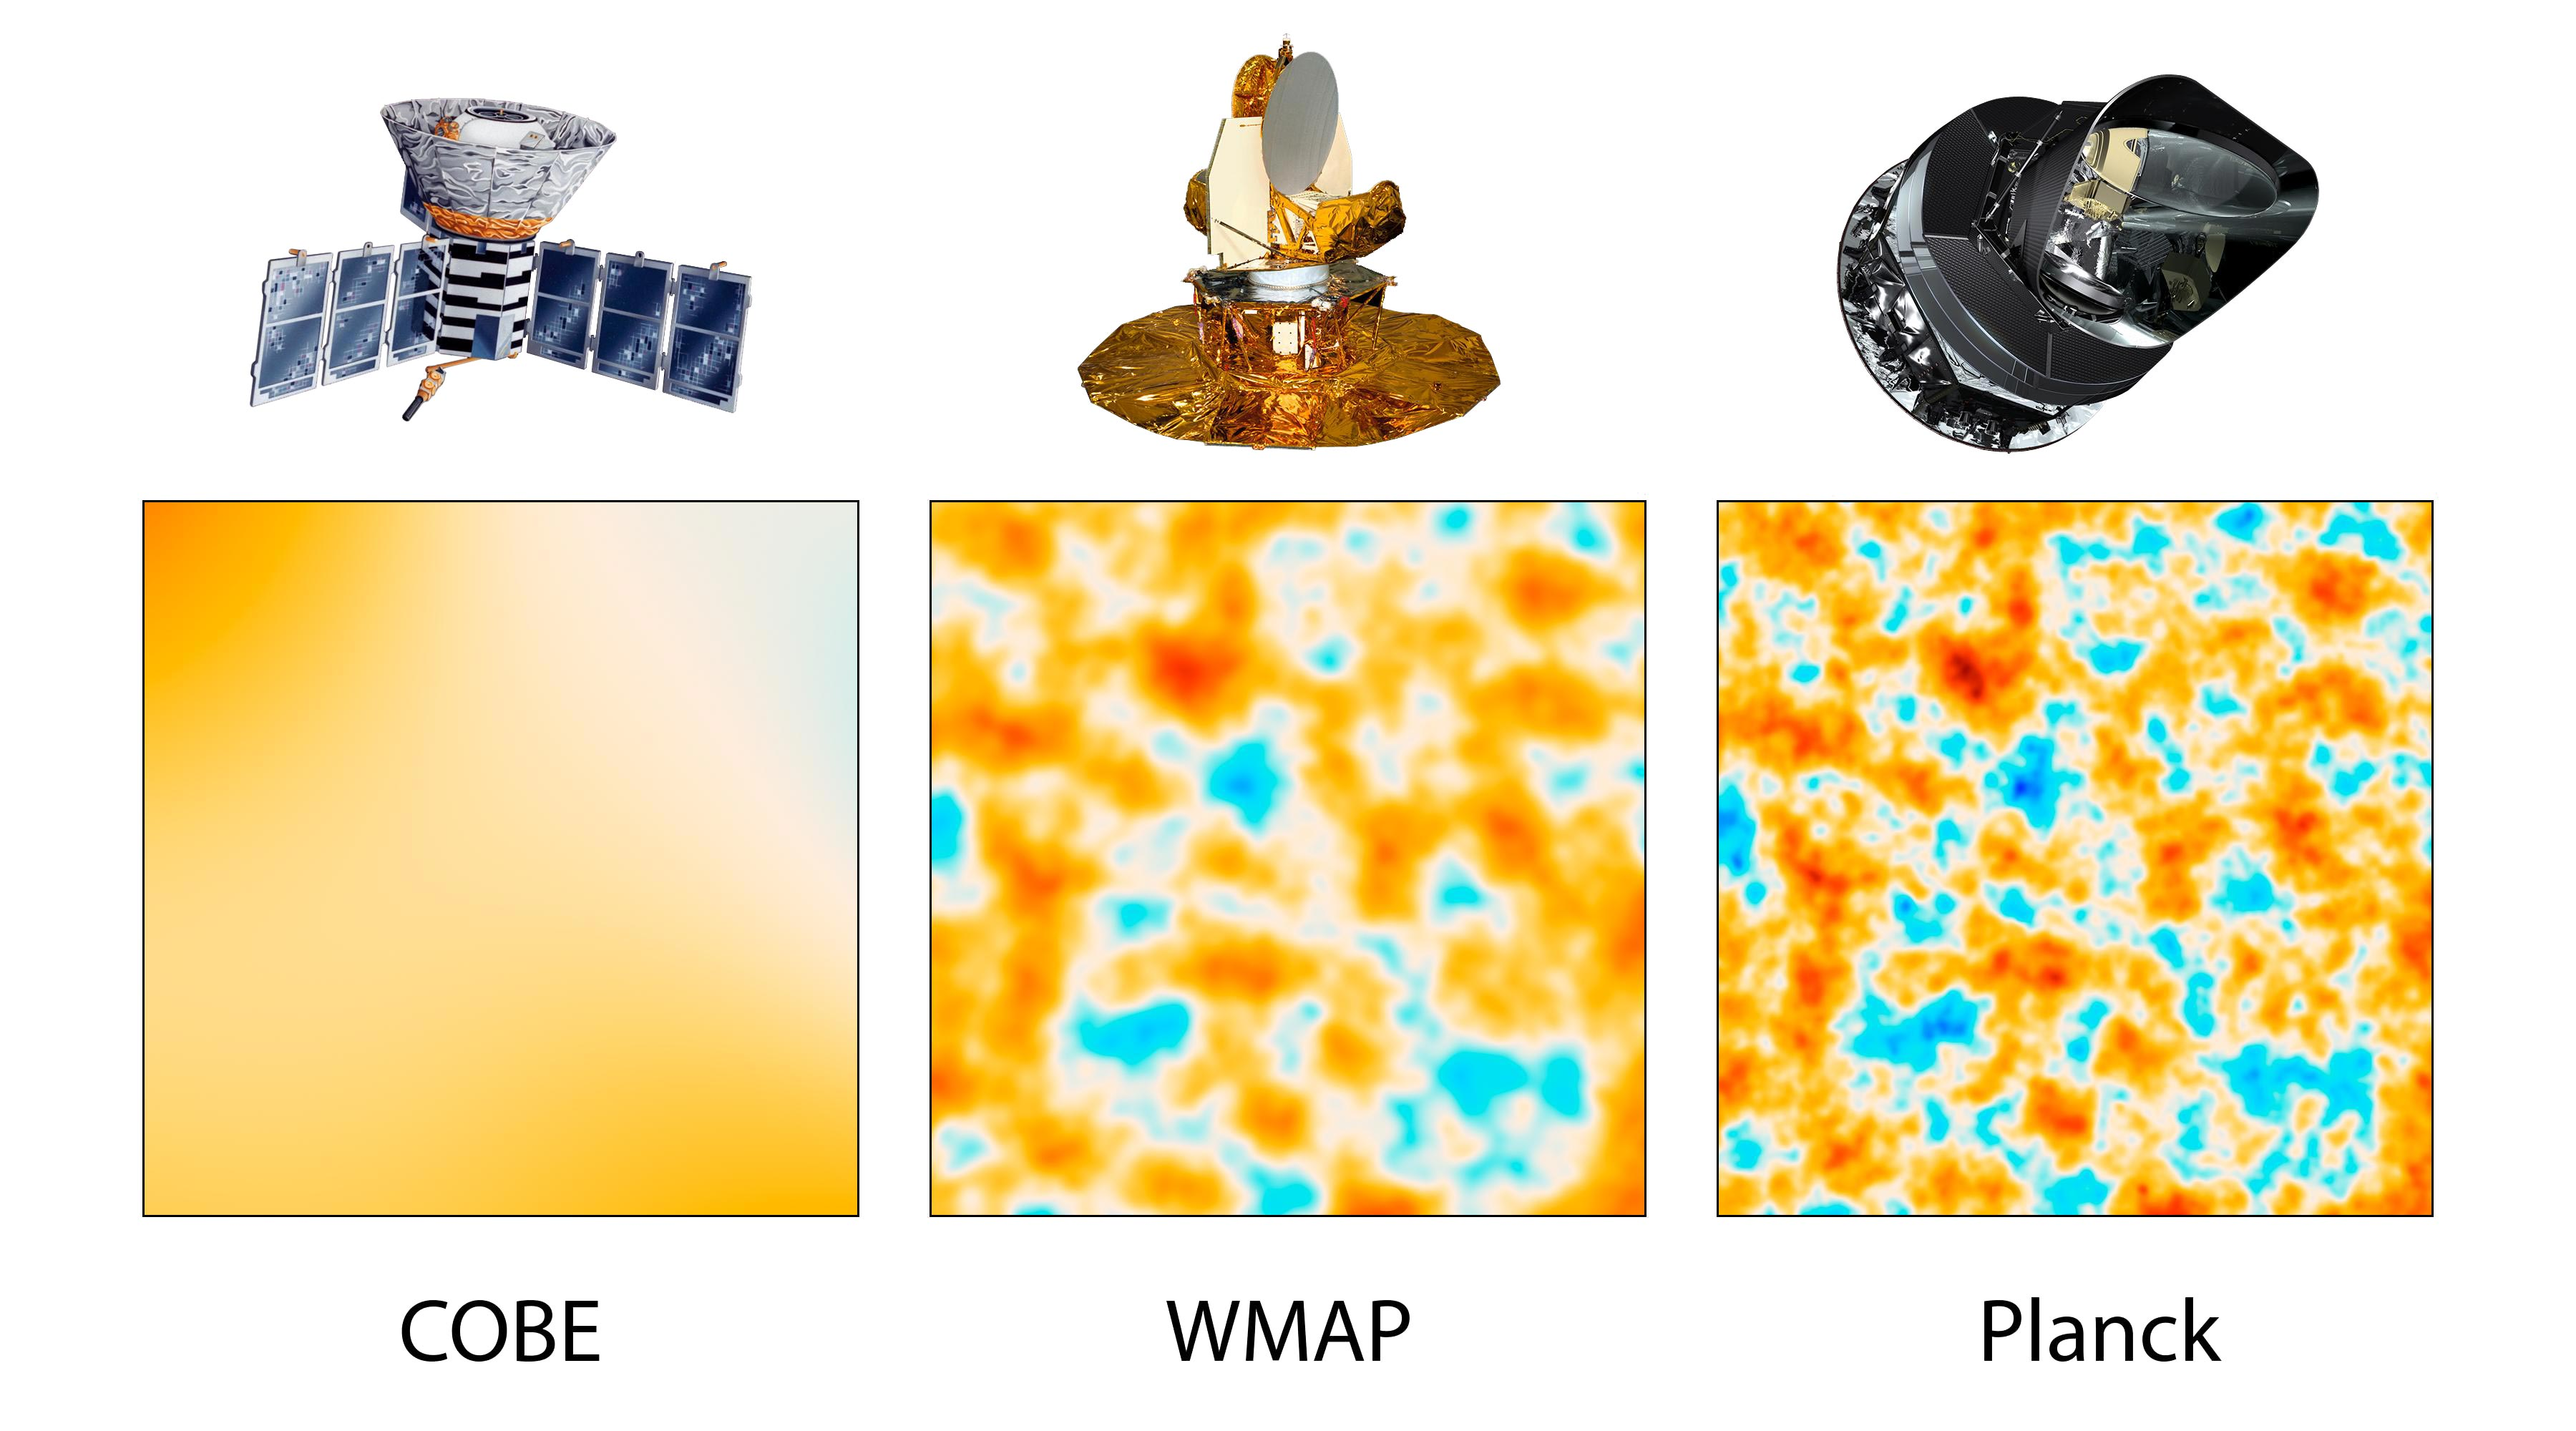
\includegraphics[width=\linewidth]{cmb/images/COBE_WMAP_Planck.jpg}
	\caption{Direkter Vergleich der aus den verschiedenen Missionen 
	entstandenen Bildern.}
	\label{fig:COBE_WMAP_PLANCK}
\end{figure}
Die Verbesserungen sind beträchtlich.
Das Bild von Planck dient auch als Grundlage für die Berechnungen, die später 
noch aufgezeigt werden.
